%Correct the file name.
%X: book number
%Y: part number
%ZZZ: page number in three digits. So page 3 would be 003.

\documentclass[11pt]{amsbook}

\usepackage{../HBSuerDemir}	% ------------------------
\renewcommand{\theequation}{\arabic{equation}}


\begin{document}

% ++++++++++++++++++++++++++++++++++++++
\hPage{b1p2/290}
% ++++++++++++++++++++++++++++++++++++++

\textbf{Example.} Obtain the standard form of the equation
\begin{equation} \label{pg290_1}
	2x^2 + 3xy - 2y^2 + 8 = 0
\end{equation}

\noindent and compute $H$, $D$ and $T$ before and after the rotation.

\textbf{Solution.} The angle of the rotation is obtained from

\begin{equation*}
	tan \ 20 = \dfrac{B}{A-C} = \dfrac{3}{2+2} = \dfrac{3}{4}
\end{equation*}

\noindent which gives
\begin{align*}
	&cos \ 20 = \dfrac{1}{\sqrt{1+tan^2 20}} = \dfrac{1}{\sqrt{1+9/16}} = 4/5 \\
	&cos \ 0 = \sqrt{\dfrac{1+cos\ 20}{2}} = \sqrt{\dfrac{1+4/5}{2}} = 3/\sqrt{10} \\
	&sin \ 0 = \sqrt{\dfrac{1-cos\ 20}{2}} = \sqrt{\dfrac{1-4/5}{2}} = 1/\sqrt{10}
\end{align*}

\noindent Then substituting
\begin{align*}
	&x = \dfrac{1}{\sqrt{10}} (3x'-y') \\
	&y = \dfrac{1}{\sqrt{10}} (x'+3y')
\end{align*}

\noindent into (\ref{pg290_1}) we have
\begin{align*}
	&2(3x'-y')^2 + \dfrac{3}{10}(3x'-y')(x'+3y') - \dfrac{2}{10}(x'+3y')^2 + 8 = 0
	\intertext{or}
	&\dfrac{2}{10}(3x'-y')^2 + 3(3x'-y')(x'+3y') - 2(x'+3y')^2 + 80 = 0 \\
	\Rightarrow \ &(18+9-2){x'}^2+(2-9-18){y'}^2+80 = 0 \\
	\Rightarrow \ &25x'^2 - 25y'^2 + 80 = 0 \Rightarrow \dfrac{{y'}^2}{80/25} - \dfrac{{x'}^2}{80/25} = 1 \Rightarrow a = b = \dfrac{4}{5}\sqrt{5}
\end{align*}

\noindent Note that
\begin{equation*}
	H = A + C = 0, \qquad H' = A' + C' = 0
\end{equation*}
\begin{align*}
	\delta = B^2-4AC = 25, \qquad \delta'=B'^2-4A'C'=-4 (\dfrac{25}{10}) (-\dfrac{25}{10}) = 25& \\
	\text{(Since F = F'= 8 for a rotation)}& \\
\end{align*}

% =======================================================
\end{document}  

%==== templates ====

%==== environments ====

%\begin{figure}[htb]
%	\centering
%	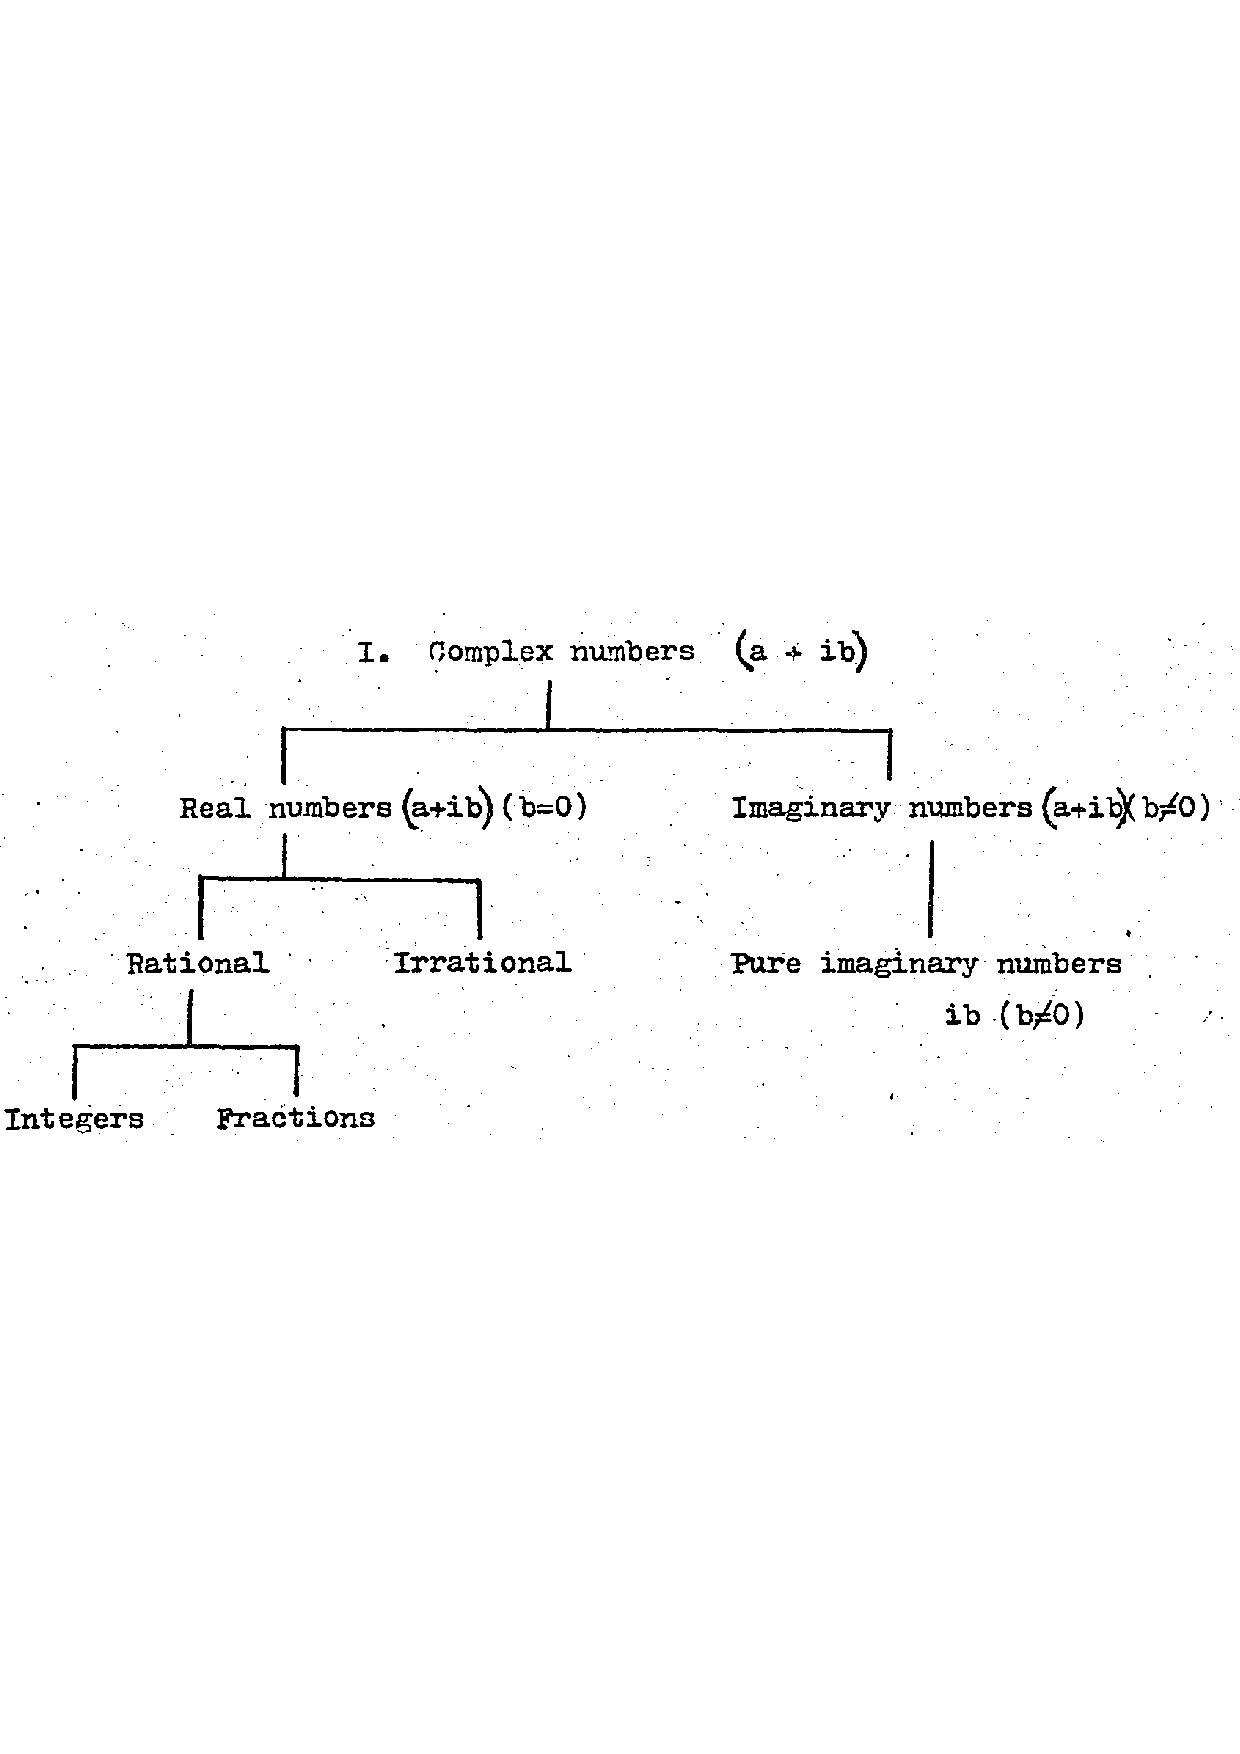
\includegraphics[width=0.9\textwidth]{images/SD-1-1p15A}
%	\caption{Classification of complex numbers}
%	\label{fig:classificationOfComplexNumbersA}
%\end{figure}

%\begin{center}
%\begin{tabular}{cc}
%\end{tabular}
%\end{center}

%\begin{exmp}
%\begin{hSolution}
%\end{hSolution}
%\end{exmp}

%\begin{hEnumerateAlpha}
%\end{hEnumerateAlpha}

%\begin{hEnumerateRoman}
%\end{hEnumerateRoman}

%$
%\begin{bmatrix}
%\end{bmatrix}
%$

%\frac{aaaa}{bbb}
%\frac{a_{n}}{b_{n}}
%\left( aaaa \right)
%\Longrightarrow

%\begin{multicols}{2}
%	bb
%\columnbreak
%	aa
%\end{multicols}
